\chapter{Base de donnée}
	\label{lab:bdd}

\section{Présentation}

Pour répondre à notre problématique de détection des lésions sur les images TEP respirantes, nous avons choisit d’utiliser une base de données d’images simulées. En effet, notre problématique repose sur une connaissance très précise de la position des lésions pour l’évaluation des performances, ainsi que sur l’acquisition de données en mode séquences. Ces deux paramètres sont très difficiles à atteindre à partir d’images cliniques.

	\subsection{Avantages des bases de données simulées}

Le principal avantage des bases de données est le contrôle qu'elles permettent d'exercer sur les modèles. Il est possible de spécifier les conditions des acquisitions de manière très précise, et permettent de garantir une homogénéité dans les conditions d'acquisitions qu'il est difficile d'atteindre en utilisant des données patient.

Dans le cadre de travaux sur la détection, la présence de la vérité terrain est un plus particulièrement appréciable, car elle permet de savoir avec une certitude impossible à atteindre en clinique la position  et le nombre des lésions. En effet, dans le cas de lésions de petit diamètre et de petit contraste, le diagnostique ne peut être donné avec une précision totale par le praticien. 

De plus, les simulations permettent d’obtenir des images avec des paramètres qui ne sont pas forcément disponibles en routine clinique. Dans notre cas, la génération des images en mode séquence est indispensable, et très peu d’examens sont réalisés de cette façon, notamment à cause de l’espace disque utilisé et des temps de reconstruction.

	\section{Modèles}

Nous avons généré utilisé une base de donnée d’images TDM fournie par le centre hospitalier Lyon-SUD pour créer 15 modèles. Cette variabilité des patients va permettre de limiter le sur-apprentissage des outils de détection. Le fantôme paramétrique XCAT~\cite{segars2009mcatoverview} développé par Paul Segars a été adapté  sur chacune des images TDM à l’aide d’un logiciel fourni, présenté dans la figure~\ref{fig:fitXCAT}. Ce modèle est basé sur des courbes paramétriques NURB (Non-Uniform Rational B-Splines). Le recalage n’est pas parfait du fait des limitations du logiciel, mais permet d’obtenir une variabilité suffisante pour notre étude. Deux images TDM associés aux fantômes adaptés sont présentés dans la figure~\ref{fig:adaptXCAT}.

\begin{figure}
 \centering
 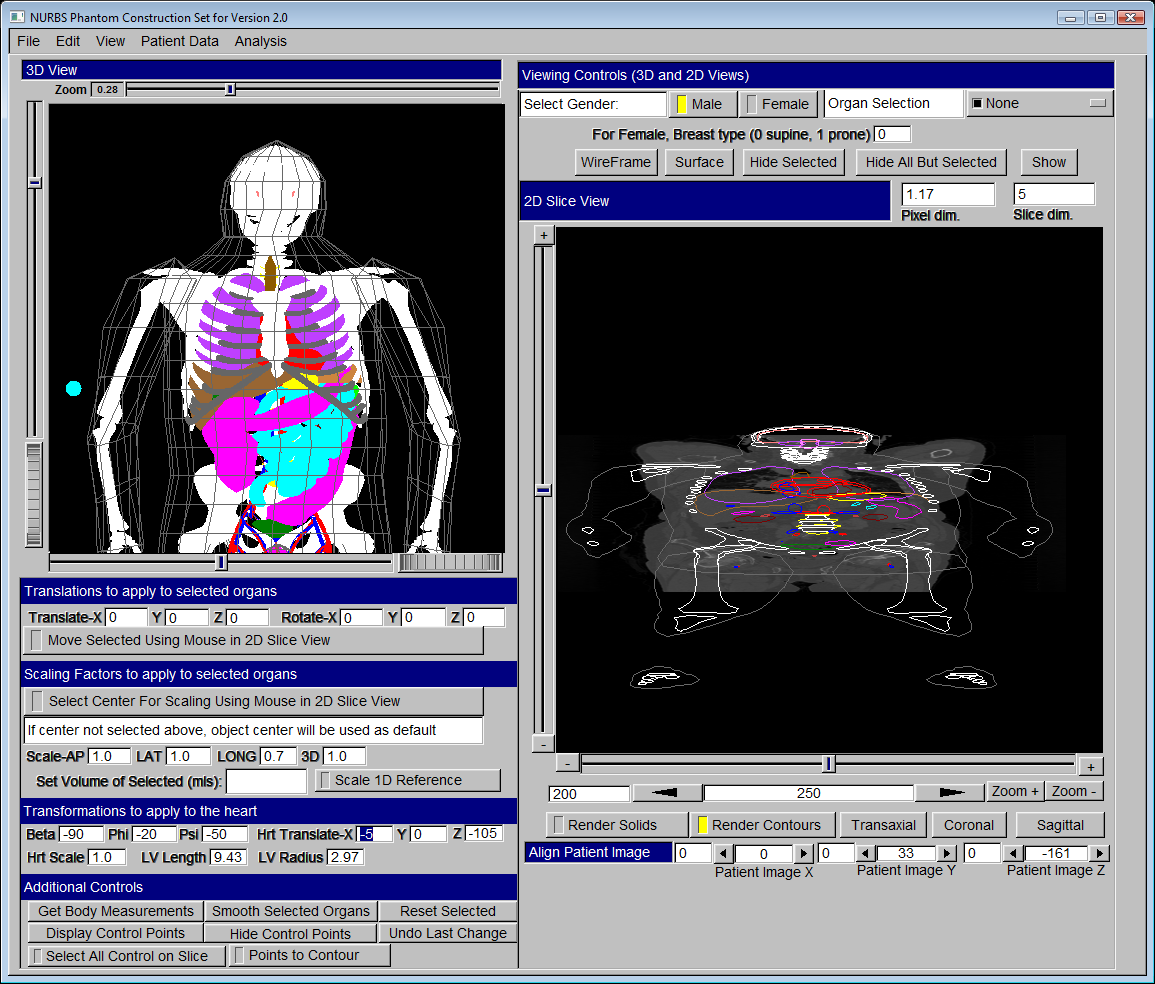
\includegraphics[width=10cm]{images/FIT_XCAT}
 \caption[Adaptation du modèle XCAT sur une image TDM de patient]{Adaptation du modèle XCAT sur une image TDM de patient : le modèle est fortement déformé par la différence entre l'épaisseur des coupes et la résolution du plan. Chaque organe est représenté par une surface paramétrique qu’il est possible d’adapter sur un modèle de patient}
 \label{fig:fitXCAT}
\end{figure}
Nous avons choisit le XCAT car il intégrait directement un modèle de mouvement respiratoire, et était conçu pour pouvoir être déformé et créer différents patients.

\begin{figure}
 \centering
 \begin{tabular}{c c}
 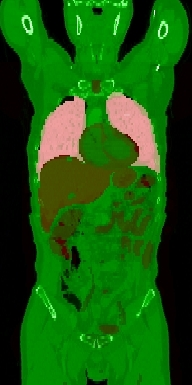
\includegraphics[width=6cm]{images/adapt_bru_jea} &
 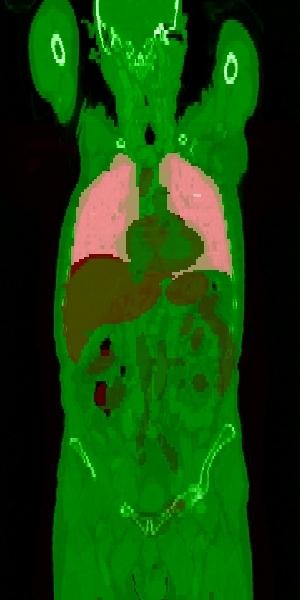
\includegraphics[width=6cm]{images/adapt_cha_chr}
 \end{tabular}
 \caption[Exemple d’adaptation d’images du modèle XCAT sur des images TDM]{ Exemple d’adaptation d’images du modèle XCAT sur des images TDM : deux modèles XCAT représentés en niveaux de rouge sont adaptés sur des images TDM représentées en vert}
 \label{fig:adaptXCAT}
\end{figure}


		\subsection{Respiration}


Pour prendre en compte la variabilité du cycle respiratoire (voir figure \ref{fig:variabCycle}), nous avons utilisé 4 cycles différents pour modéliser la respiration du patient. Un signal respiratoire complet a été acquis sur une durée de plusieurs minutes à l'aide d'un spiromètre (voir \ref{lab:spirometre}). Nous avons extraits 3 cycles semblables correspondants à la phase de de respiration normale, ainsi qu'un cycle ``anormal'' pour prendre en compte une respiration irrégulière.

\begin{figure}
 \centering
 \begin{tabular}{c c}
 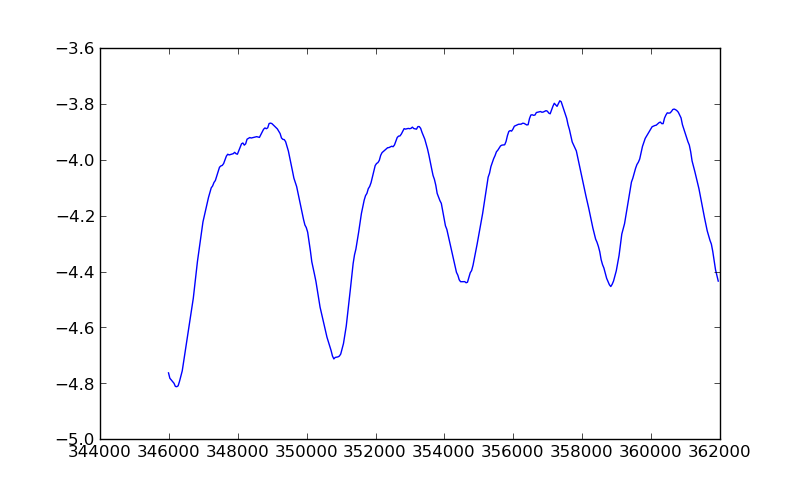
\includegraphics[width=8cm]{images/respiReguliere} &
 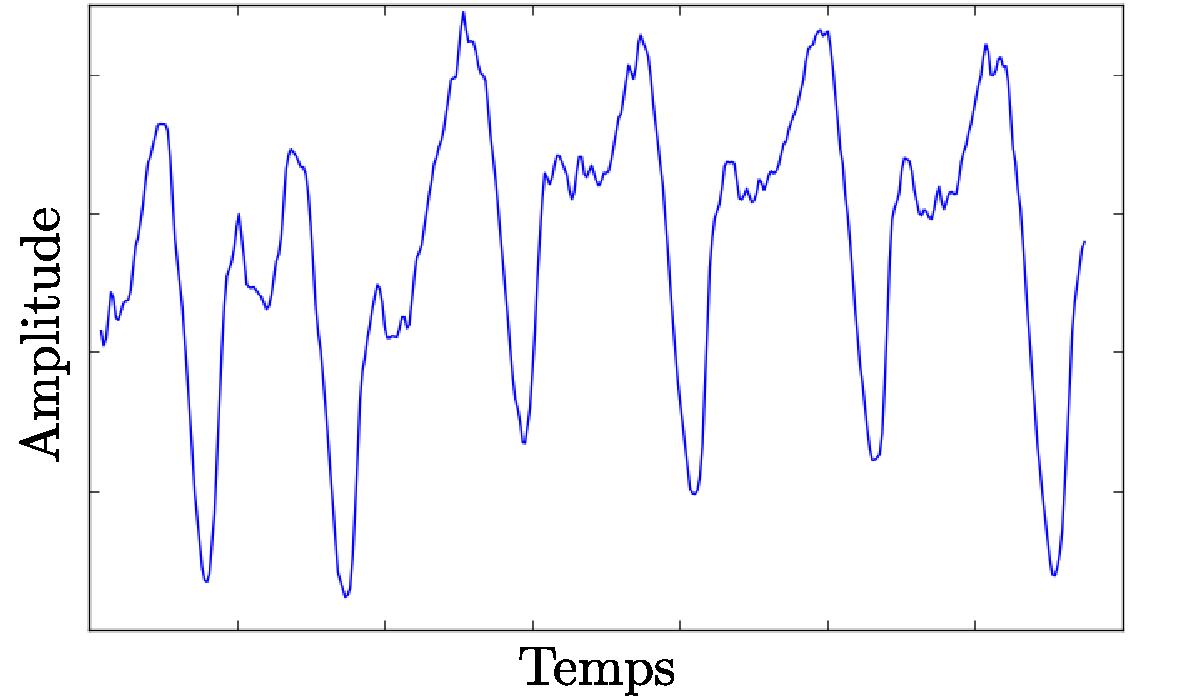
\includegraphics[width=8cm]{images/respiIrreguliere}
 \end{tabular}
 \caption[Exemple de courbes respiratoires régulière et irrégulière]{Deux exemples de courbes respiratoires prises par un spiromètre : celle de gauche montre une respiration régulière, tandis que celle de droite est irrégulière}
 \label{fig:variabCycle}
\end{figure}


La signal respiratoire obtenue est présentée dans la figure \ref{fig:cycleRespi}. Il est constitué de 4 cycles de 5.6 secondes qui se répètent 10 fois pour former un signal total de 224 secondes. 

Chacun de ces 4 cycles est discrétisé en 8 parties qui seront utilisées pour générer les modèles utilisés lors de la simulation. 


\begin{figure}
 \centering
 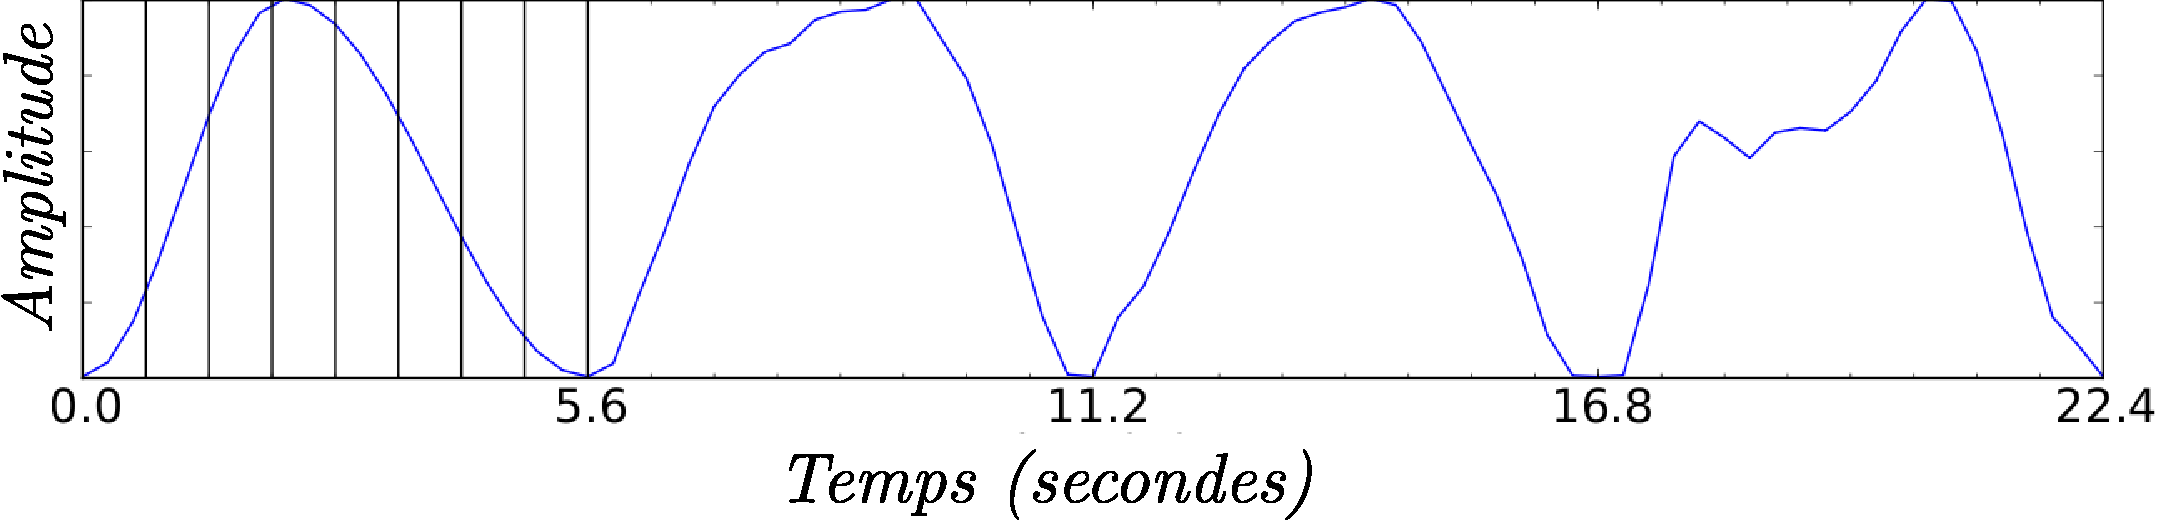
\includegraphics[width=8cm]{images/courbesRespi}

 \caption[signal respiratoire utilisé pour les modèles de la base de donnée]{Courbe respiratoire utilisée pour générer modèles respirant. Les traits verticaux du premier cycle montrent les 8 instants sélectionnés pour discrétiser le mouvement respiratoire de ce cycle.}
 \label{fig:cycleRespi}
\end{figure}

	\section{paramètres de simulation}

\subsection{Calibration de la base de données}

Notre but est de simuler des images avec un ensemble de tumeurs qui ne soient ni trop évidentes ni impossible à détecter. Nous avons donc cherché à obtenir une échelle de contrastes de tumeurs qui permettaient une détection par des humains de 10\%, 30\%, 50\%, 70\% et 90\%.

Pour réaliser cela, un ensemble d'images ont été simulées sans mouvement respiratoire, avec différentes tailles de tumeurs. Ensuite, une étude ROC avec deux observateurs humains non médecin est réalisée afin d'estimer la détectabilité de ces couples activité/taille de tumeurs (fig.\ref{fig:calibration}). 

Nous avons utilisé la base de donnée crée dans notre laboratoire et présentée dans~\cite{tomei2010oncopet_db}. Cette base de donnée contient entre autre 25 images TEP simulées à partir du modèle zubal~\cite{zubal1994computerized}, contenant 10 lésions par image. Ces lésions sont placées de manière aléatoire dans le poumon, les ganglions lymphatiques, le foie et la rate avec une probabilité de 30\% pour les 3 premiers organes et de 10\% pour la rate. Le contraste de ces lésions est déjà calibré pour une détection sur une échelle de 10\% à 90\%. Il y a donc 250 lésions, 75 dans les ganglions lymphatiques, 75 dans le foie, 75 dans le poumon, et 25 dans la rate. Nous n'avons réalisé notre étude que sur le foie et le poumon.

On présente à chaque observateur les images les unes après les autres, qu'ils vont annoter en recherchant toutes les lésions et en leur attribuant une note à l'aide du logiciel amide~\cite{loening2003amide}. Ils ne connaissent pas à l'avance la localisation des lésions, et doivent donner pour chaque lésion une note entre 1 et 5 correspondant au barème suivant :

\begin{enumerate}
\item Possible
\item Probable
\item Très probable
\item Pratiquement  certain
\item Certain
\end{enumerate}

\subsubsection{Étude de détectabilité}

Nous avons utilisé la base de donnée originale, avec les contrastes présentés en \ref{tab:contrastePoumonOrig} pour les lésions du poumon et \ref{tab:contrasteFoieOrig} pour les lésions du foie.

\begin{table}
\centering
\begin{tabular}{|c||c|c|c|c|c|}
 \hline
Poumon	& 10\% & 30\% & 50\% & 70\% & 90\% \\
\hline
4mm	& 2    &  5   &  8   & 10   & 13   \\
\hline
12mm    & 2    &  5   &  8   & 10   & 13   \\
\hline
16mm    & 2    &  3.5 &  4.5 & 7.5  & 10   \\
\hline
\end{tabular}

\caption[Contraste originaux des lésions du poumon pour létude de détectabilité]{Contrastes originaux appliqués aux lésions de la base OncoPET\_DB pour les tumeurs du poumon, avec les pourcentages de détection associés}
\label{tab:contrastePoumonOrig}
\end{table}

\begin{table}
\centering

\begin{tabular}{|c||c|c|c|c|c|}
 \hline
Poumon	& 10\% & 30\% & 50\% & 70\% & 90\% \\
\hline
4mm	& 2.5    &  4   &  4.5   & 6   & 9   \\
\hline
12mm    & 2    &  3   &  4   & 4.5   & 7.5   \\
\hline
16mm    & 2    &  3   &  4   & 4.5   & 7.5   \\
\hline
\end{tabular}

\caption[Contraste originaux des lésions du foie pour létude de détectabilité]{Contrastes originaux appliqués aux lésions de la base OncoPET\_DB pour les tumeurs du foie, avec les pourcentages de détection associés}
\label{tab:contrasteFoieOrig}
\end{table}

Lors de cette première étude, nous avons observé que les lésions de la base de données étaient beaucoup trop visibles, ce qui nous a amené à redéfinir les contrastes à utiliser pour la nouvelle version de la base de donnée. 


Les figures \ref{fig:calibrationFoie} et \ref{fig:calibration} représentent respectivement le taux de détection des lésions du foie et du poumon lors de l'étude de détectabilité les lésions réalisée sur la base d'origine.


\begin{figure}[h!]
\begin{center}
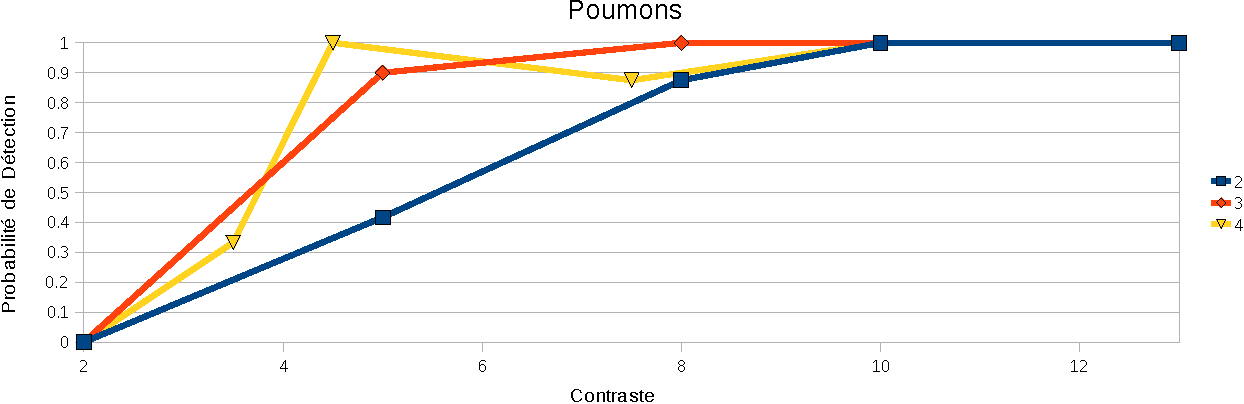
\includegraphics[width=15cm]{images/calibration_crop}
\end{center}
\caption{Détectabilité des tumeurs du poumon réalisées par des humains en fonction du contraste et de la taille des tumeurs. Chaque courbe représente une taille de lésion différente} 
\label{fig:calibration}
\end{figure}

\begin{figure}[h!]
\begin{center}
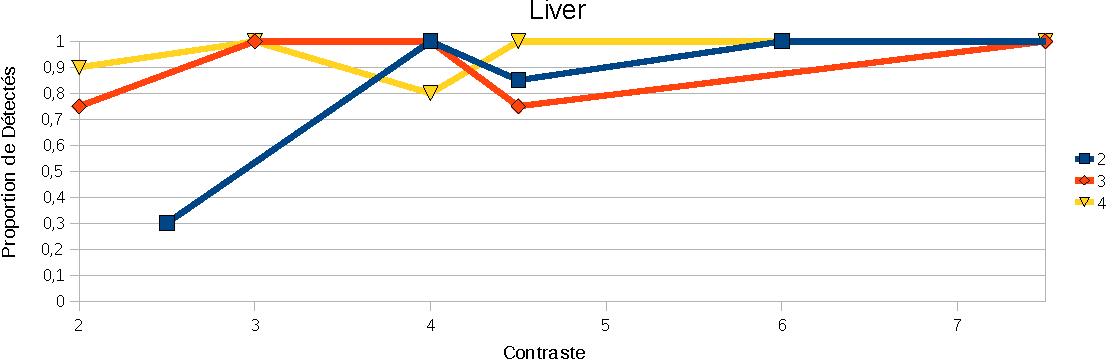
\includegraphics[width=15cm]{images/calibrationFoie_crop}
\end{center}
\caption{Détectabilité des tumeurs du foie réalisées par des humains en fonction du contraste et de la taille des tumeurs. Chaque courbe représente une taille de lésion différente} 
\label{fig:calibrationFoie}
\end{figure}




\begin{table}
\centering

Poumon :\\
\begin{tabular}{|c|c|c|c|}
 \hline
 Détection voulue & 	8mm & 	12mm & 	16mm \\
\hline
90 \%		  & 100 \%  & 100 \% & 100 \% \\
\hline
70 \%		  & 100 \%  & 100 \% & 90 \%\\
\hline
50 \%		  & 90 \%  & 100 \% & 100 \%\\
\hline
30 \%		  & 44 \%  & 90 \% & 30 \%\\
\hline
10 \% 		  & 0 \%  & 0 \% & 0 \%\\
\hline
\end{tabular}

\vspace{0.5cm}


Foie :\\
\begin{tabular}{|c|c|c|c|}
 \hline
 Détection voulue & 	8mm & 	12mm & 	16mm \\
\hline
90 \%		  & 100 \%  & 100 \% & 100 \% \\
\hline
70 \%		  & 100 \%  & 75 \% & 100 \%\\
\hline
50 \%		  & 85 \%  & 100 \% & 75 \%\\
\hline
30 \%		  & 100 \%  & 100 \% & 100 \%\\
\hline
10 \% 		  & 30 \%  & 75 \% & 90 \%\\
\hline

\end{tabular}

\caption[Détectabilité estimée des lésions en fonction du contraste et de leur diamètre]{Détectabilité des lésions réalisée à l'aide d'une étude par des humains. La colonne de gauche indique la détectabilité supposée des lésions.}
\label{fig:detectabiliteVue}
\end{table}

En pratique, les résultats de la figure~\ref{fig:detectabiliteVue} montrent une détectabilité largement supérieure à celle indiquée. Après étude du tableau, il s'avère que les lésions de 16 mm sont trop visibles pour être intégrées dans l'étude. Nous avons fait des interpolations linéaires entre les statistiques obtenues pour définir les nouvelles activités, définies en \ref{tab:contrasteFoieFinal} pour le foie et le poumon.



\begin{table}

\centering

\begin{tabular}{|c||c|c||c|c|}
 \hline
	& 8mm Foie	& 12mm Foie	& 8mm Poumon	& 12mm Poumon	\\
\hline
10\%	& 1.8		& 1.3		& 3.0		& 2.5		\\
\hline
30\%	& 2.0		& 1.5		& 4.0		& 3.0		\\
\hline
50\%	& 2.5		& 1.8		& 5.0		& 3.5		\\
\hline
70\%	& 3.0		& 2.0		& 6.5		& 4.0		\\
\hline
90\%	& 3.5		& 2.3		& 8.0		& 5.0		\\
\hline
\end{tabular}
\caption[Contraste final lésions du foie et du poumon]{Contrastes appliqués aux lésions en fonction du taux de détectabilité désiré}
\label{tab:contrasteFoieFinal}
\end{table}



\section{Optimisation des paramètres de simulation}

L'optimisation des paramètres de reconstruction a été réalisée à partir d'une étude sur le rapport signal sur bruit des lésions.

Nous avons cherché le jeu de paramètres (Nombre d'itérations, Nombre de sous-ensemble) qui permettais de maximiser ce critère sur les images.

\section{Types d'images générées}

La base de données générée contient 15 patients, reconstruits avec une correction parfaite (image statique), sans correction, et avec deux méthodes de correction du mouvement respiratoire présentées en \ref{lab:corrPostRecon} et \ref{lab:CorrpendantRecon}. Un exemple d'images de la base est visible dans la figure~\ref{fig:exempleImageRecon}.

\begin{figure}
 \centering
 
\includegraphics[width=10cm]{images/exempleImageRecon}
 \caption[Images reconstruites tirées de la base de donnée]{Images reconstruites tirées de la base de donnée. La flèche représente une lésion du poumon de diamètre 8mm avec une activité de niveau 5.}
 \label{fig:exempleImageRecon}
\end{figure}

\subsection{Images Statiques}

Les images statiques sont reconstruites à partir des donnés de simulation statiques, réalisées à partir d'une acquisition complète du modèle au premier instant du cycle respiratoire (fin d'expiration).

Elle est donc en phase avec la carte d'atténuation qui est elle aussi tirée du modèle en fin d'expiration.

\subsection{Images Non corrigées}

Les images non corrigées sont produites de la même manière que les images statiques, mais à partir des fichiers séquence dynamiques.

\subsection{Estimation du mouvement respiratoire}

Pour estimer le mouvement respiratoire, nous avons décidé d'utiliser les images TEP, car cette technique nous permet d'ajouter une imprécision réaliste. Les données dynamiques sont utilisées pour la reconstruction.

Les 8 images correspondant aux 8 instants du cycle moyen sont reconstruites séparément sans correction d'atténuation. Nous réalisons ensuite un recalage de chaque image sur l'image de référence (la première) à l'aide d'un algorithme de recalage élastique par B-splines. Le recalage est réalisé dans les deux sens, de manière à éviter de devoir inverser un des champs de mouvement.

Les champs de mouvement estimés vont permettre la correction du mouvement des images. 

Pour permettre une meilleure adéquation des données dynamiques avec la carte d'atténuation, elle est déformée à l'aide des champs de mouvement pour correspondre aux différents instants du cycle respiratoire.

\subsection{Images TE-MS}

Ces images sont reconstruites à l'aide d'un logiciel fourni par le LatIM~\cite{lamare2007list}, qui prend en compte l'estimation de mouvement réalisée précédemment ainsi que les fichiers list-mode générés par la simulation dynamique pour reconstruire directement les images corrigées. Les 8 cartes d'atténuation déformées sont fournies de manière à réaliser une reconstruction optimale.

\subsection{Images TI-IM}

Les 8 images correspondant aux 8 instants du cycle moyen sont reconstruites séparément à l'aide de la carte d'atténuation recalée correspondante. Puis toutes ces images sont déformées sur l'image correspondant au premier instant du cycle à l'aide de la carte de mouvement estimée précédemment.

Ces 8 cartes recalées sont ensuite sommées pour obtenir les images corrigées.


	\section{données clef} % temps de calculs etc....

\subsection{Lésions}

\begin{table}
\centering
 \begin{tabular}{|c|c||c|c|c|c|c|} 
\hline
\multicolumn{2}{|c|}{Niveau de confiance}       & 1	  & 2	    & 3	     & 4	& 5	\\
\hline
\hline
Poumon	(173)	& 8 mm (90)	& 3 (19)  & 4 (18)  & 5 (18)  & 6.5 (18)	& 8 (17)\\
\cline{2-7}
		& 12 mm	(83)	& 2.5 (16)& 3 (16)  & 3.5 (18)& 4 (17)	& 5 (16)\\
\hline
Foie 	(107)	& 8 mm (54)		& 1.8 (11)& 2 (11)  & 2.5 (10)& 3 (11)	& 3.5 (11)\\
\cline{2-7}
		& 12 mm	(53)	& 1.3 (10)& 1.5 (10)& 1.8 (11)& 2 (11)  & 2.3 (11)\\
\hline 
 \end{tabular}

\caption[Tableau récapitulatif des lésions]{Tableau récapitulatif des contrastes des lésions présentes dans le foie et les poumon des modèles. Le nombre en parenthèse correspond au nombre de lésions}
\label{tab:contrastePoumonFoieRecap}


\end{table}

\subsection{activité des organes}


Les activités des organes sont décrites dans la table \ref{tab:contrastePoumonFoieRecap}. Elles ont été estimées à partir d'une étude réalisée précédemment lors des travaux de thèse de Sandrine Tomeï, en mesurant l'activité dans des zones d'intérêt présentes dans les organes.

\begin{table}
\centering
 \begin{tabular}{|c|c|c|} 
\hline
Organe 		& Activité ($Bq/c^3$) \\
\hline
\hline
Foie		& 7740		       \\
\hline
Myocarde	& 11610		       \\
\hline
Os		& 3863		       \\
\hline
Poumon 		& 1338 		       \\
\hline
Prostate	& 2575		       \\
\hline
Rate		& 4939		       \\
\hline
Reins		& 8220		       \\
\hline
Sang		& 5340		       \\
\hline
Tissus mous 	& 2575 		       \\
\hline
Urètre		& 33815		       \\
\hline
Vésicule bilaire& 2575		       \\
\hline
Vessie		& 50973		       \\
\hline
 \end{tabular}

\caption[Activités des organes des patients de la base de donnée]{Activités définies pour les organes des patients virtuels}
\label{tab:activiteOrganes}
\end{table}

Nous avons crée 15 modèles, qui ont été adaptés depuis autant d'images TDM fournies par le centre hospitalier Lyon-SUD. Nous avons utilisé pour cela les outils fournis par Paul Segars~\cite{segars2001These}.

Les images sont reconstruites avec des voxels de 4mm dans les trois dimensions. Les reconstructions sont réalisées à l'aide de l'algorithme OPL-EM avec 8 itérations complètes et 5 sous-ensembles, sauf pour l'estimation de mouvement où seulement 3 itérations complètes avec 5 subsets sont réalisées, avec une régularisation de 6mm à chaque itération. 

Le temps de simulation nécessaire pour générer une image statique est de 130h par processeur environ, et 110 heures pour générer une image dynamique.

Le volume de données généré est d'environ 6Go par patient sans prendre en compte les données intermédiaires générées lors de la simulation.
